\section{Weitere Prinzipien (8P)}
\subsection{Analyse GRASP: Geringe Kopplung (3P)}
\task{eine bis jetzt noch nicht behandelte Klasse als positives Beispiel geringer Kopplung; UML mit zusammenspielenden Klassen, Aufgabenbeschreibung der Klasse und Begründung, warum hier eine geringe Kopplung vorliegt; es müssen auch die Aufrufer/Nutzer der Klasse berücksichtigt werden}
Die Klasse CategoryRestController ist für die Anbindung der CRUD-Endpunkte für den HTTP-Server für alle Kategorien eines Nutzers. Sie hat eine geringe Kopplung da sie nur für CRUD-Endpunkte für Kategorien dar sind. Davor waren alle Endpunkte im MainRestController. 
\newline\newline
\begin{figure}[htbp]
    \centering
    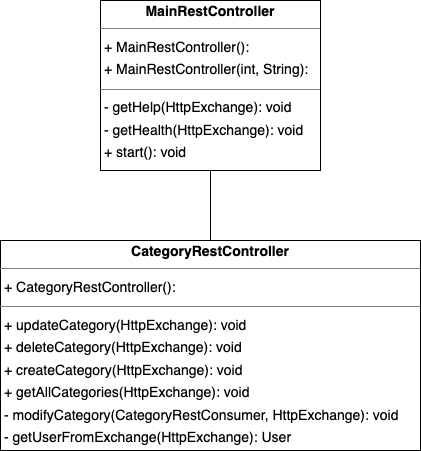
\includegraphics[width=0.75\linewidth]
    {kapitel4_other_principals/grasp.png}
\end{figure}

\subsection{Analyse GRASP: [Polymorphismus/Pure Fabrication] (3P)}
\task{eine Klasse als positives Beispiel entweder von Polymorphismus oder von Pure Fabrication; UML Diagramm und Begründung, warum es hier zum Einsatz kommt}
Damit alle Commands gleich sind und keine Methoden fehlen wurde ein Interface geschrieben, welches jeder Command erbt.  
\newline\newline
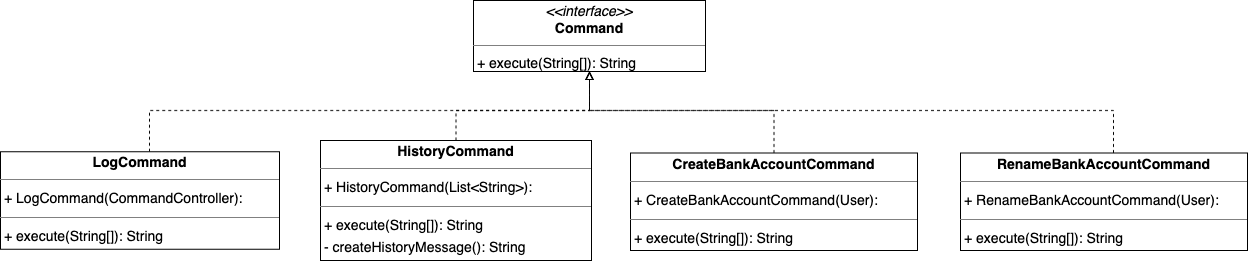
\includegraphics[width=\linewidth]{kapitel4_other_principals/grasp_poly.png}
\subsection{DRY (2P)}
\task{ein Commit angeben, bei dem duplizierter Code/duplizierte Logik aufgelöst wurde; Code-Beispiele (vorher/nachher) einfügen; begründen und Auswirkung beschreiben – ggf. UML zum Verständnis ergänzen}

Branch: \textit{main/Commit bc6ad15} 
\subsubsection*{Vorher}
\lstinputlisting[language=Java,style=codeStyle]{kapitel4_other_principals/before.java}
\subsubsection*{Nachher}
\lstinputlisting[language=Java,style=codeStyle]{kapitel4_other_principals/after.java}
\subsubsection*{Beschreibung}
Es gab viele Methoden die, denn selben Code in einer kleinen abgeänderten Art ausgeführt haben. Die Lösung war eine Methode namens \textit{convertCurrency(String currencyCode, String currencyName)} die in den einzelnen Methoden für die jeweilige Währung aufgerufen wird. 
\todo{Beschreiben warum die Namen der Währungen gehartcoded sind (ggf. Alternativen aufzeigen)}
\newline\newline
Das hatte zur Folge das der Code einfacherer zu lesen ist und unnötige Codezeilen gespart werden konnten. 
